\chapter{Results of the Cross Section Measurement}
The cross-sections are calculated as described in Chap.~\ref{chap:Met}. All of the W cross-sections are summarized in Tab. \ref{tab:Wcs}.  The total uncertainty of the measurements in the fiducial region consists of the statistical, systematical and luminosity errors. The methods of these uncertainties determination are described in Chap. \ref{chap:Unc}.

Because of the lepton universality of the Standard Model, the results, obtained in electron and muon channel are expected to agree with each other. The ratio in electron and muon channel is calculated with the respect of the correlated systematic uncertainties is shown in Fig.\ref{fig:LeptUnivers}. The ratios errors are mostly dominated by the statistics on the W and Z samples and agrees with Standard Model predictions within the uncertainty.

\begin{figure}[!b]
\begin{center}
\begin{minipage}[h]{0.8\linewidth}
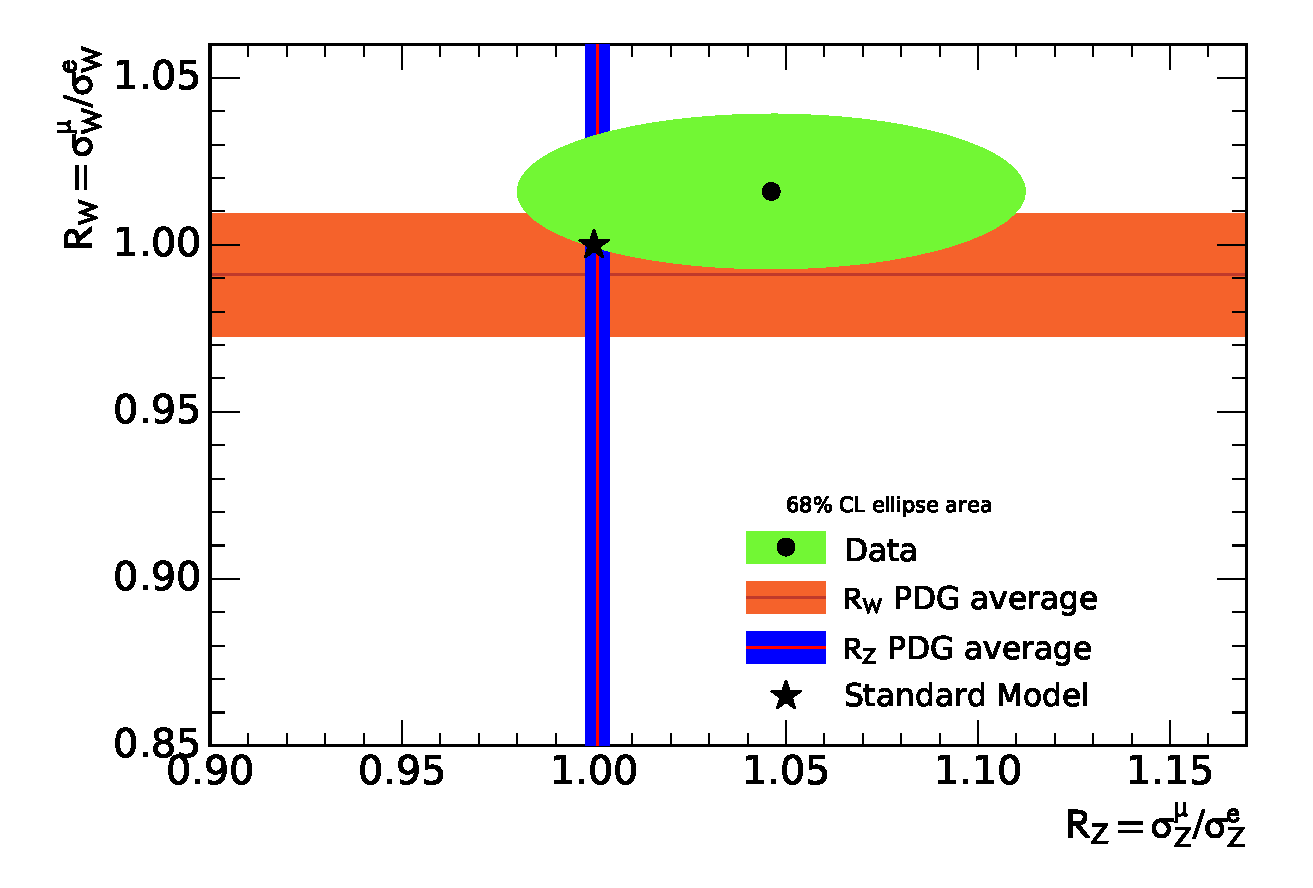
\includegraphics[width=1\textwidth]{Results/Univers.pdf}
\end{minipage}
\caption{Ratio of Z and W-boson production fiducial cross sections obtained in electron electron and muon channel compared to the expectations of the Standard Model and previous experimental checks of the lepton universality provided as PDG average bands.}
\label{fig:LeptUnivers}
\end{center}
\end{figure}

\begin{table}[!tb]
\caption{Results on a fiducial $\sigma^{fid}$ and total cross-section measurement for $W^{+}$, $W^{-}$ and Z bosons in electron and muon channels. The cross-sections are shown with their statistical, systematical and luminosity uncertainties (and extrapolation error for total cross-section) quoted in that order}
\label{tab:Wcs}
\begin{center}
\begin{tabular}{| l | c | c |}
\hline
 & value $\pm$ stat $\pm$ syst $\pm$ lumi ($\pm$ ext)& value $\pm$ stat $\pm$ syst $\pm$ lumi ($\pm$ ext) \\
 \hline
 \hline
 & \multicolumn{2}{c|}{W in electron channel}\\
& $W^{+}\to e\nu$ & $W^{-}\to e\nu$ \\

\hline
$\sigma^{fid}_{W}$ [pb]  & \sigfidWplusenunolabel & \sigfidWminenunolabel \\
$\sigma^{tot}_{W}$ [pb] & \sigtotWplusenunolabel & \sigtotWminenunolabel \\
$\sigma^{13}_{W}$ [pb] & \sigTrWplusenunolabel & \sigTrWminenunolabel \\
\hline
\hline
 & \multicolumn{2}{c|}{W in muon channel}\\
& $W^{+}\to \mu\nu$ & $W^{-}\to \mu\nu$\\
\hline
$\sigma^{fid}_{W}$ [pb] & \sigfidWplusmununolabel & \sigfidWminmununolabel \\
$\sigma^{tot}_{W}$ [pb]  & \sigtotWplusmununolabel & \sigtotWminmununolabel \\
$\sigma^{13}_{W}$ [pb]  & \sigTrWplusmununolabel & \sigTrWminmununolabel \\
\hline
%\hline
 %& \multicolumn{2}{c|}{$W^{+-}$ } \\
%& $W \to e\nu$ & $W \to \mu \nu$ \\
%\hline
%$\sigma^{fid}_{W}$ &  & \\
%$\sigma^{tot}_{W}$ & & \\
%$\sigma^{13}_{W}$ & & \\
%\hline
\hline
 & \multicolumn{2}{c|}{Z} \\
& $Z \to ee$ & $ Z \to \mu\mu$ \\
\hline
$\sigma^{fid}_{Z}$  [pb] &\sigfidZeenolabel &  \sigfidZmumunolabel \\
$\sigma^{tot}_{Z}$  [pb] & \sigtotZeenolabel & \sigtotZmumunolabel \\
$\sigma^{13}_{Z}$ [pb]  & \sigTrZeenolabel & \sigTrZmumunolabel \\
\hline
\end{tabular}
\end{center}
\end{table}
\section{Combined results}

Since the results between channels are agreeing well, it is possible to perform averaging as described in Sec. \ref{sec:Aver}. Systematic uncertainties for the averaging are taken from Tab. \ref{tab:Unc}. The systematic uncertainties calculated using Toy MC are included in the averaging following the prescription from Sec. \ref{sec:Cor}. The common luminosity uncertainty is excluded from the combination process. The systematic uncertainties from electroweak background sources are considered uncorrelated between W and Z bosons and 100\% correlated for different W and Z channels.

The combination yields a good $\chi^2/NDF$=1.0/3 indicating good agreement between measurements. The combined cross-section is extrapolated to the full fiducial phase-space using $A_{W/Z}$ factors. The resulting cross-sections are summarized in Tab. \ref{tab:csComb}.
\begin{table}[!tb]
\caption{Results on a fiducial $\sigma^{fid}$ and total cross-section measurement for $W^{+}$, $W^{-}$ and Z bosons in electron and muon channels. The cross-sections are shown with their statistical, systematical and luminosity uncertainties (and extrapolation error for total cross-section) quoted in that order}
\label{tab:csComb}
\begin{center}
\begin{tabular}{| l | c | c |}
\hline
 & value $\pm$ stat $\pm$ syst $\pm$ lumi ($\pm$ ext)& value $\pm$ stat $\pm$ syst $\pm$ lumi ($\pm$ ext) \\
 \hline
 \hline
 & \multicolumn{2}{c|}{$W^{+/-}$}\\
& $W^{+}\to l\nu$ & $W^{-}\to l\nu$ \\

\hline
$\sigma^{fid}_{W}$ [pb]  & $\valfidWp \pm \statfidWp \pm \sysfidWp \pm \lumifidWp$ & $\valfidWm \pm \statfidWm \pm \sysfidWm \pm \lumifidWm$ \\
$\sigma^{tot}_{W}$ [pb] & $\valfullWp \pm \statfullWp \pm \sysfullWp \pm \lumifullWp \pm \extrfullWp$ & $\valfullWm \pm \statfullWm \pm \sysfullWm \pm \lumifullWm \pm \extrfullWm$ \\
$\sigma^{13}_{W}$ [pb] & $\valthrWp \pm \statthrWp \pm \systhrWp \pm \lumithrWp$ & $\valthrWm \pm \statthrWm \pm \systhrWm \pm \lumithrWm$ \\
\hline
\hline
& \multicolumn{2}{c|}{$W \to l \nu$} \\
\hline
$\sigma^{fid}_{W}$ [pb] & \multicolumn{2}{c|}{$\valfidWtot \pm \statfidWtot \pm \sysfidWtot \pm \lumifidWtot$} \\
$\sigma^{tot}_{W}$ [pb]  & \multicolumn{2}{c|}{$\valfullWtot \pm \statfullWtot \pm \sysfullWtot \pm \lumifullWtot \pm \extrfullWtot$} \\
$\sigma^{13}_{W}$ [pb]  & \multicolumn{2}{c|}{$\valthrWtot \pm \statthrWtot \pm \systhrWtot \pm \lumithrWtot$} \\
\hline
%\hline
 %& \multicolumn{2}{c|}{$W^{+-}$ } \\
%& $W \to e\nu$ & $W \to \mu \nu$ \\
%\hline
%$\sigma^{fid}_{W}$ &  & \\
%$\sigma^{tot}_{W}$ & & \\
%$\sigma^{13}_{W}$ & & \\
%\hline
\hline
 & \multicolumn{2}{c|}{$Z \to ll$} \\
\hline
$\sigma^{fid}_{Z}$ [pb] & \multicolumn{2}{c|}{$\valfidZ \pm \statfidZ \pm \sysfidZ \pm \lumifidZ$} \\
$\sigma^{tot}_{Z}$ [pb]  & \multicolumn{2}{c|}{$\valfullZ \pm \statfullZ \pm \sysfullZ \pm \lumifullZ \pm \extrfullZ$} \\
$\sigma^{13}_{Z}$ [pb]  & \multicolumn{2}{c|}{$\valthrZ \pm \statthrZ \pm \systhrZ \pm \lumithrZ$} \\
\hline
\end{tabular}
\end{center}
\end{table}

\section{Cross-sections ratios}
The combination cross-section are in a fiducial region:
\begin{itemize}
\item $R_{W/Z} = \valfidWZ \pm \statfidWZ \, (stat)\, \pm \sysfidWZ\, (sys)\,  $
\item $R_{W^{+}/Z} = \valfidWpZ \pm \statfidWpZ\, (stat)\, \pm \sysfidWpZ \, (sys)\, $
\item $R_{W^{-}/Z} = \valfidWmZ \pm \statfidWmZ\, (stat)\,  \pm \sysfidWmZ\,  (sys)\, $
\item $R_{W^{+}/W^{-}} = \valfidWpWm \pm \statfidWpWm\, (stat)\, \pm \sysfidWpWm\,  (sys)\,  $
\end{itemize}


\section{Comparation with Theoretical Predictions}
The theoretical predictions for cross-section measurements are obtained at NLO using MCFM/APPLIGRID for a different PDF sets: ABM12nlo, CT14nlo, MMHTnlo, ATLAS-epWZnlo, HERAPDF2.0nlo. 
\section{PDF fits}